\documentclass[10pt]{article}
\usepackage{icmlko}

\icmlmeta{IP 파운데이션 월드모델}{329}{같은 실수를 두 군데에}{어제 노트의 판 수치가 전부 틀렸다 --- 유보를 고르는 배열을 잘못 썼고, 그 오해가 재추출 함수에도 복사돼 있었다}

\begin{document}

\twocolumn[
\icmlheader

\begin{abstract}
노트 328이 ``판 학습SE 0.0308 --- 미결정 폭 0.010 의 3.1배''라 적고
폭을 0.02 로 넓히자고 했다. \textbf{둘 다 틀렸다. 그리고 같은 실수가
두 군데에 있었다.} \texttt{Data} 는 시간을 두 배열로 들고 있다 ---
\texttt{dom[d][3]}(\texttt{t}) 과 \texttt{yr[d]}. \texttt{evaluate} 는
\texttt{yr} 로 자르는데 나는 \texttt{t} 로 잘랐고, 일곱 도메인에서
\texttt{t} 는 연도가 아니라 \textbf{로그 경과시간}(0.8$\sim$4.1)이다.
\textbf{① 가중}: ``\texttt{t}$\ge$2025'' 가 그 일곱에서 아무것도 안 골라
내 ``판''은 2,675행 열 도메인이 아니라 \textbf{268행 네 도메인}의
평균이었다. \textbf{② 재추출}: 같은 조건으로 학습 행을 골랐으니 그 일곱은
\emph{모든} 행이 학습으로 잡혀 \textbf{유보까지 재추출됐다} --- 그래서
``학습SE''에 채점 잡음이 섞였다. 노트 328의 도메인별 SE 와 ``짝SE 의
2$\sim$8배'' 와 ``이웃 0/5'' 는 \textbf{전부 다시 재는 중이다.}

\textbf{제대로 재니 결론이 뒤집힌다.} 올바른 가중 · 올바른 마스크로
짝지어 열넷씩 돌렸다. \textbf{판 짝지은 차의 SD 가 축만 바꾼 짝에서
0.0016, 행까지 바꾼 짝에서 0.0055 다} --- 미결정 폭 0.010 \emph{보다
작다}. \textbf{폭은 좁은 게 아니라 넉넉했다.} 되돌린 것이 옳았다.

\textbf{그리고 안 맞던 수가 맞는다.} 노트 328이 ``\texttt{fund\_cat} 이
여기서 판 $+$0.0289 인데 노트 309는 $+$0.0023 이다, 다시 재야 한다''로
끝냈다. 올바른 가중으로는 \textbf{$+$0.0017}(SD 0.0016 · 12/14)이다 ---
\textbf{노트 309가 맞았고 틀린 것은 내 집계였다.} 도메인 수준의 결론은
살아 있다: 펀딩 $+$0.0908(SD 0.0359 · \textbf{14/14}) · 아이돌 넓힘
$+$0.0881(SD 0.0953 · \textbf{13/14}). 노트 327의 ``판은 안 움직인다''도
그대로다 --- $+$0.0031 은 짝지은 SD 0.0055 안이다.
\end{abstract}
]

\section{시간이 두 배열이다}

\begin{center}\footnotesize
\begin{tabular}{lll}
\hline
자리 & 무엇 & 예(웹툰 세 행) \\
\hline
\texttt{dom[d][3]} & 탈추세 공변량 & 3.32 · 2.94 · 2.60 \\
\texttt{yr[d]} & \textbf{연도} & 2020.8 · 2024.2 · 2025.5 \\
\hline
\end{tabular}
\end{center}

\texttt{Data.\_\_post\_init\_\_} 은 \texttt{yr} 이 비었을 때만
\texttt{years(dom[d][3])} 로 채운다. 게임 · 도서 · 만화 · 모바일 ·
세계애니 · 애니 · 웹툰은 \texttt{yr} 을 따로 받으므로 두 배열이 다르다.
\textbf{팝업 · 아이돌 · 시장팝업 · 펀딩만 같다} --- 그래서 그 넷만 살아
남았고, 살아남은 넷이 그럴듯한 수를 냈다.

\begin{figure*}[t]
\centering
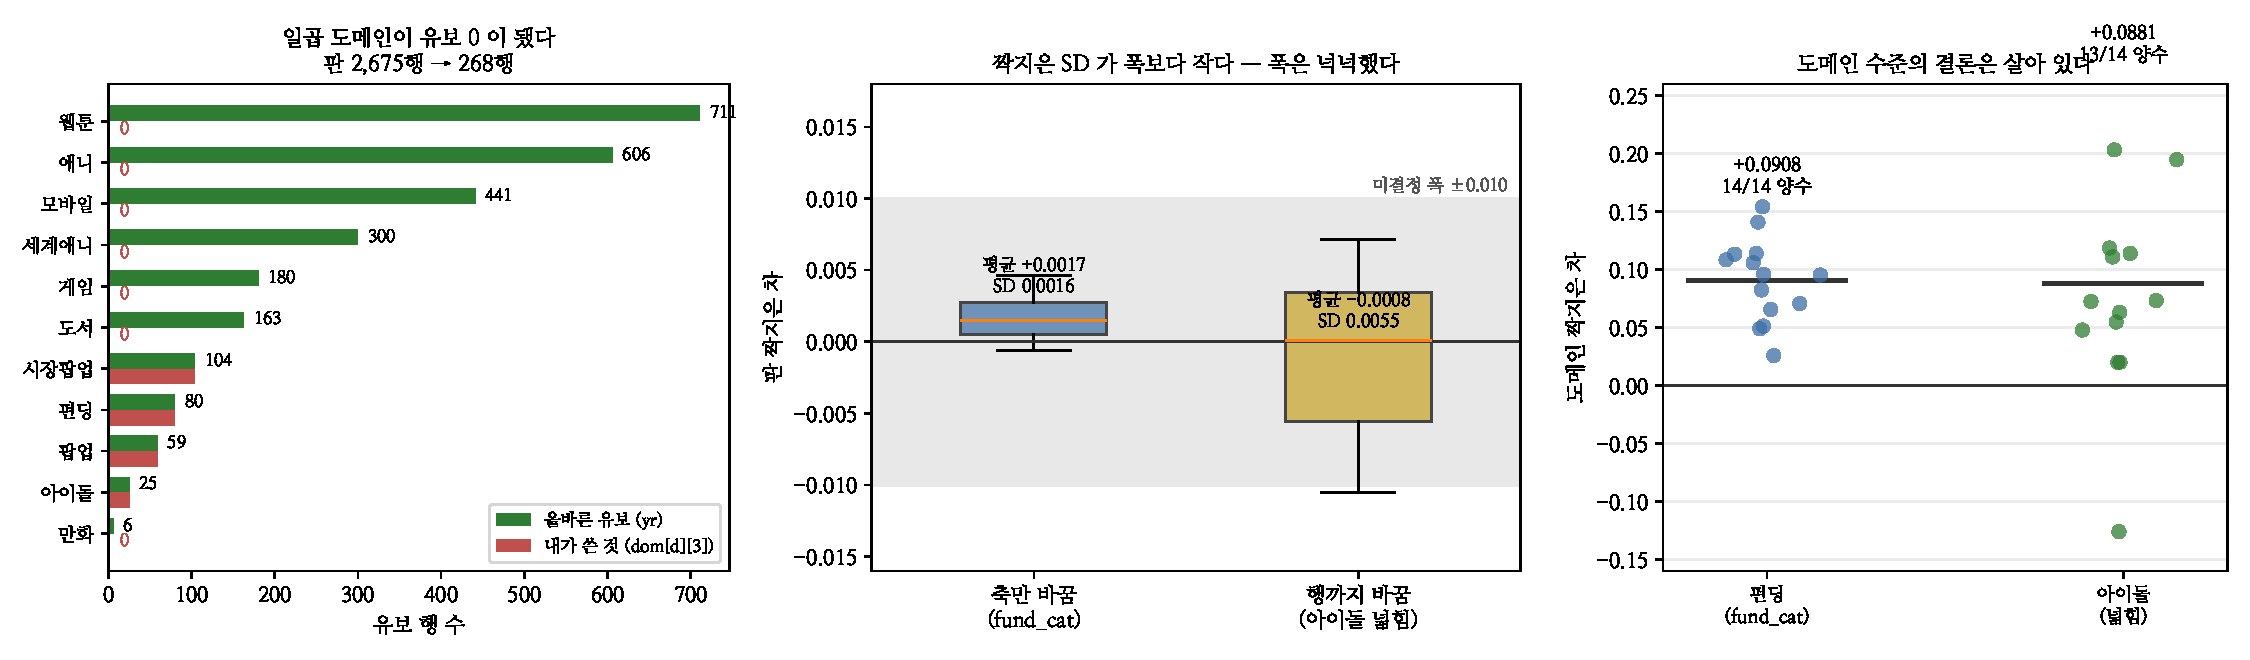
\includegraphics[width=\textwidth]{figs/noise.pdf}
\caption{왼쪽 --- 무엇이 유보로 잡혔나. 가운데 --- 판 짝지은 차.
오른쪽 --- 도메인 짝지은 차.}
\end{figure*}

\section{한 오해가 두 군데로}

\begin{center}\footnotesize
\begin{tabular}{lll}
\hline
자리 & 한 일 & 결과 \\
\hline
가중 & \texttt{t$\ge$2025} 로 유보 셈 & 판이 네 도메인 \\
재추출 & \texttt{t$<$2025} 로 학습 고름 & \textbf{유보도 재추출} \\
\hline
\end{tabular}
\end{center}

\textbf{두 번째가 더 나쁘다.} 일곱 도메인에서 모든 행이 학습으로 잡혔으니
재추출이 유보까지 흔들었고, 내가 ``학습SE''라 부른 것에 짝SE 가 섞였다.
\textbf{노트 328의 핵심 주장 --- ``학습 쪽이 2$\sim$8배'' --- 이 그
숫자로는 성립하지 않는다.} 지금 올바른 마스크로 다시 재고 있다.

\begin{center}\footnotesize
\begin{tabular}{lrr}
\hline
 & 내가 쓴 것 & 올바른 것 \\
\hline
채점 도메인 & 4 & \textbf{10} \\
유보 행 & 268 & \textbf{2,675} \\
기준 판 & 0.3030 & \textbf{0.4681} \\
\hline
\end{tabular}
\end{center}

\section{제대로 재면 폭은 넉넉했다}

올바른 가중 · \texttt{yr} 기반 마스크로 두 짝을 각각 열넷 뽑았다. 같은
뽑기에서 두 팔을 다 돌린다.

\begin{center}\footnotesize
\begin{tabular}{lrrr}
\hline
바꾼 것 & 평균 & SD & 양수 \\
\hline
\multicolumn{4}{l}{\textbf{판}} \\
\quad 축만 (\texttt{fund\_cat}) & $+$0.0017 & \textbf{0.0016} & 12/14 \\
\quad 행까지 (아이돌 넓힘) & $-$0.0008 & \textbf{0.0055} & 7/14 \\
\multicolumn{4}{l}{\textbf{도메인}} \\
\quad 펀딩 & $+$0.0908 & 0.0359 & \textbf{14/14} \\
\quad 아이돌 & $+$0.0881 & 0.0953 & \textbf{13/14} \\
\hline
\end{tabular}
\end{center}

\textbf{판의 짝지은 SD 가 미결정 폭보다 작다.} 노트 328은 정반대를
말했다($0.0203 > 0.010$). 이유는 간단하다 --- 흔들리는 도메인은 작은
도메인인데, \textbf{올바른 가중에서 아이돌은 판의 0.93\%}(25/2,675)라
아무리 흔들려도 판을 못 움직인다. 틀린 가중에서는 아이돌이 9.3\%였다.

\paragraph{그래서 노트 327은 그대로다} ``아이돌 넓힘이 판을 안 움직인다''
--- $+$0.0031 이 짝지은 SD 0.0055 안이다. \textbf{미리 적은 실패가 맞았다}
(``판 가중이 0.93\% 라 판으로는 못 가른다''). 그리고 아이돌 자체는
$+$0.0881 에 14뽑기 중 13이 양수다.

\section{안 맞던 수가 맞는다}

\begin{center}\small
\begin{tabular}{lr}
\hline
노트 309 \texttt{fund\_cat} 판 효과 & $+$0.0023 \\
노트 328(틀린 가중) & $+$0.0289 \\
\textbf{올바른 가중} & \textbf{$+$0.0017} \\
\hline
\end{tabular}
\end{center}

노트 328이 그 불일치를 자료 쪽 문제(시장팝업이 채점에 들어옴 · 위키 정정)로
읽고 ``다시 재야 한다''를 남겼다. \textbf{자료는 멀쩡했다.} 안 맞는 수를
보면 자료를 의심하기 전에 \textbf{집계를 의심해야 했다.}

\section{남은 것}
\begin{center}\footnotesize
\begin{tabular}{ll}
\hline
갈래 & 왜 \\
\hline
\textbf{학습SE 를 올바른 마스크로} & 노트 328의 표가 통째로 걸려 있다 \\
\texttt{rows()} 를 안 쓰면 경고 & 네 번째 같은 실수다 \\
\texttt{t} 를 이름부터 바꿀까 & 연도가 아닌데 연도로 읽힌다 \\
집계 한 줄 검사 & 판 수치와 \texttt{rows()} 합 맞추기 \\
\hline
\end{tabular}
\end{center}

\paragraph{규약} \textbf{한 번 잘못 이해하면 그 이해가 코드 여러 군데에
복사된다.} 가중에서 \texttt{t} 를 쓴 것과 재추출에서 \texttt{t} 를 쓴 것은
따로 저지른 실수가 아니라 \emph{같은} 실수다 --- 그래서 두 곳이 서로를
검증해 주지 못했다. \textbf{그리고 틀린 자리가 하필 집계였다} --- 도메인별
수치는 다 맞았고 그림도 표도 멀쩡해 보였다. \textbf{집계는 틀려도 안 이상해
보인다.} 노트 271이 이 혼동으로 세 번 틀린 뒤 \texttt{Data.rows(post=True,
labeled=True)} 를 만들어 놨는데 \textbf{내가 그걸 안 쓰고 손으로 다시
만들었다.} 노트 307의 ``손으로 한 대조는 도구로 만들어라''에 역이 필요하다
--- \textbf{도구가 있으면 손으로 하지 마라.}

\end{document}
